\section{组成架构}

如\cref{fig:graph_db_architecture}所示, 一般图数据库的架构主要分为接口,计算和存储三个层级。



\subsection{接口层: API与查询语言}

接口层是用户与图数据库系统之间的交互接口, 主要包括API和查询语言. API (应用程序接口) 使得开发者可以通过编程语言与数据库进行交互, 执行各种操作, 如增、删、改、查等. 图数据库通常支持多种查询语言, 如Neo4j的\textbf{Cypher}语言、Apache TinkerPop的\textbf{Gremlin}等. 这些查询语言使得用户能够方便地对图数据进行复杂的查询和分析. 接口层的设计直接关系到系统的易用性和灵活性.


\subsection{计算层: 查询引擎与优化器}

计算层负责处理用户的查询请求, 包括查询的解析、优化和执行. 查询引擎接收用户通过接口层提交的查询请求, 并将其转化为可以执行的查询计划. 优化器则对查询计划进行优化, 以提高查询的执行效率. 图数据库的查询引擎需要处理大量节点和边的遍历, 因此其性能在很大程度上决定了数据库的整体表现. 高效的查询引擎和优化器是保证复杂图查询能够在合理时间内完成的关键.

\begin{figure}[H]
	\centering
	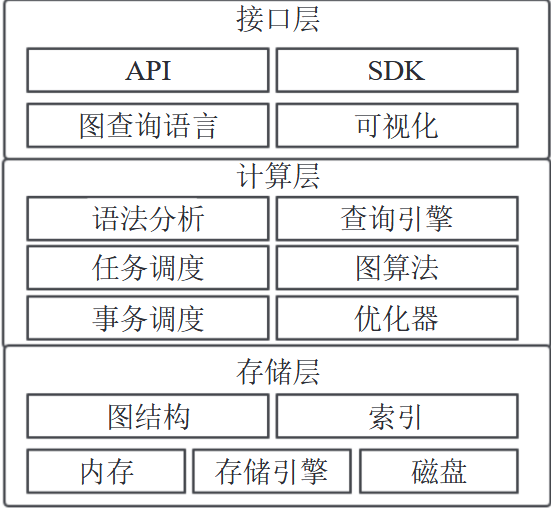
\includegraphics[width=0.6\textwidth]{images/3.png}
	\caption{图数据库的组成架构}
	\label{fig:graph_db_architecture}
\end{figure}

\subsection{存储层: 原生图存储与非原生图存储}

存储层是图数据库的基础, 负责存储节点、边及其属性. 根据实现方式的不同, 图数据库的存储层可以分为原生图存储和非原生图存储.
原生图存储是专门为图数据设计的存储结构, 能够直接以图的形式存储数据, 查询时可以高效地进行节点和边的遍历操作, 代表性的产品有Neo4j. 这种存储方式能够充分利用图数据的特性, 提供高效的存储和查询性能.
非原生图存储则是基于已有的通用数据库系统 (如关系型数据库或键值存储) 实现的图存储. 这种方式通过将图数据映射到关系型表格或键值对中来进行存储, 虽然实现成本较低, 但在查询图结构数据时效率较低, 典型的产品有JanusGraph. 这种存储方式适合一些对查询效率要求不高, 或已有存储系统需要扩展支持图数据的场景.
